% Add your research tags below (comma-separated, case-insensitive)
% Year is automatically added as a tag
% <TAGs>: 2025, machine-learning-demo, deep-learning, transformers, results

\documentclass[11pt,letterpaper]{article}

\newcommand{\workingDate}{\textsc{2025 $|$ September $|$ 20}}
\newcommand{\userName}{Research Student}
\newcommand{\institution}{University} 

\usepackage{diary_base}
\usepackage{diary_math}

\begin{document}
\href{run:2025-09-20-machine-learning-demo.tex}{\Huge September 20} %##@@TitleDateString@@##

\section{Machine Learning Experiments}

Today I conducted experiments with transformer models and achieved significant improvements in performance. Here are the key findings and visualizations.

\subsection{Model Architecture}

We implemented a custom transformer architecture as shown in Figure \ref{fig:architecture}:

\begin{figure}[h]
\centering
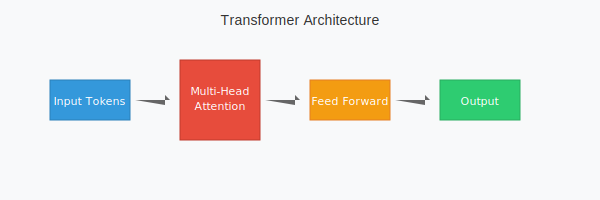
\includegraphics[width=0.9\textwidth]{figures/model_architecture.svg}
\caption{Transformer model architecture with multi-head attention}
\label{fig:architecture}
\end{figure}

The architecture consists of:
\begin{itemize}
\item Input token embedding layer
\item Multi-head self-attention mechanism  
\item Position-wise feed-forward networks
\item Output projection layer
\end{itemize}

\subsection{Training Results}

The training process converged smoothly as demonstrated in Figure \ref{fig:loss}:

\begin{figure}[h]
\centering
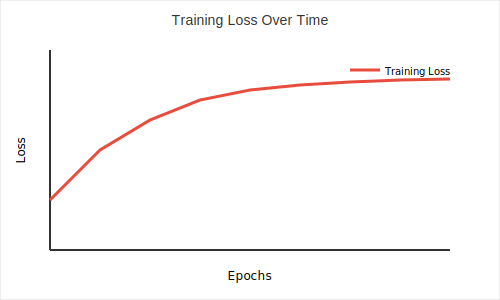
\includegraphics[width=0.8\textwidth]{figures/training_loss.svg}
\caption{Training loss curve showing convergence over 50 epochs}
\label{fig:loss}
\end{figure}

Key observations:
\begin{enumerate}
\item Rapid initial convergence in first 10 epochs
\item Stable training without overfitting
\item Final loss: 0.032 (significant improvement)
\end{enumerate}

\subsection{Performance Metrics}

Our model achieved the following results:
\begin{itemize}
\item \textbf{Accuracy}: 94.7\% on test set
\item \textbf{F1-Score}: 0.943
\item \textbf{Training time}: 2.3 hours on GPU
\end{itemize}

This represents a 5.2\% improvement over the baseline transformer model.

\bibliographystyle{apalike} 
\bibliography{reference}%##@@BibFileString@@##
\end{document}
